\section{Design, Modeling, and Analysis}

\subsection{Feature Model}

Following EAST-ADL methodology, we begin with a feature model (Fig.~\ref{fig:features}) defining system variability. The root feature \textit{CanFillingSystem} has four mandatory features: \textit{DetectCanPosition}, \textit{ControlLiquidFlow}, \textit{MonitorFillLevel}, and \textit{LogOperations}. Sensor type selection uses an XOR constraint between \textit{UltrasonicSensor} and \textit{CapacitiveSensor}. We selected ultrasonic for better reliability across liquid types. Two optional features, \textit{FaultDetection} and \textit{EmergencyShutdown}, are included with \textit{requires} dependency between them.

\begin{figure}[htbp]
\centering
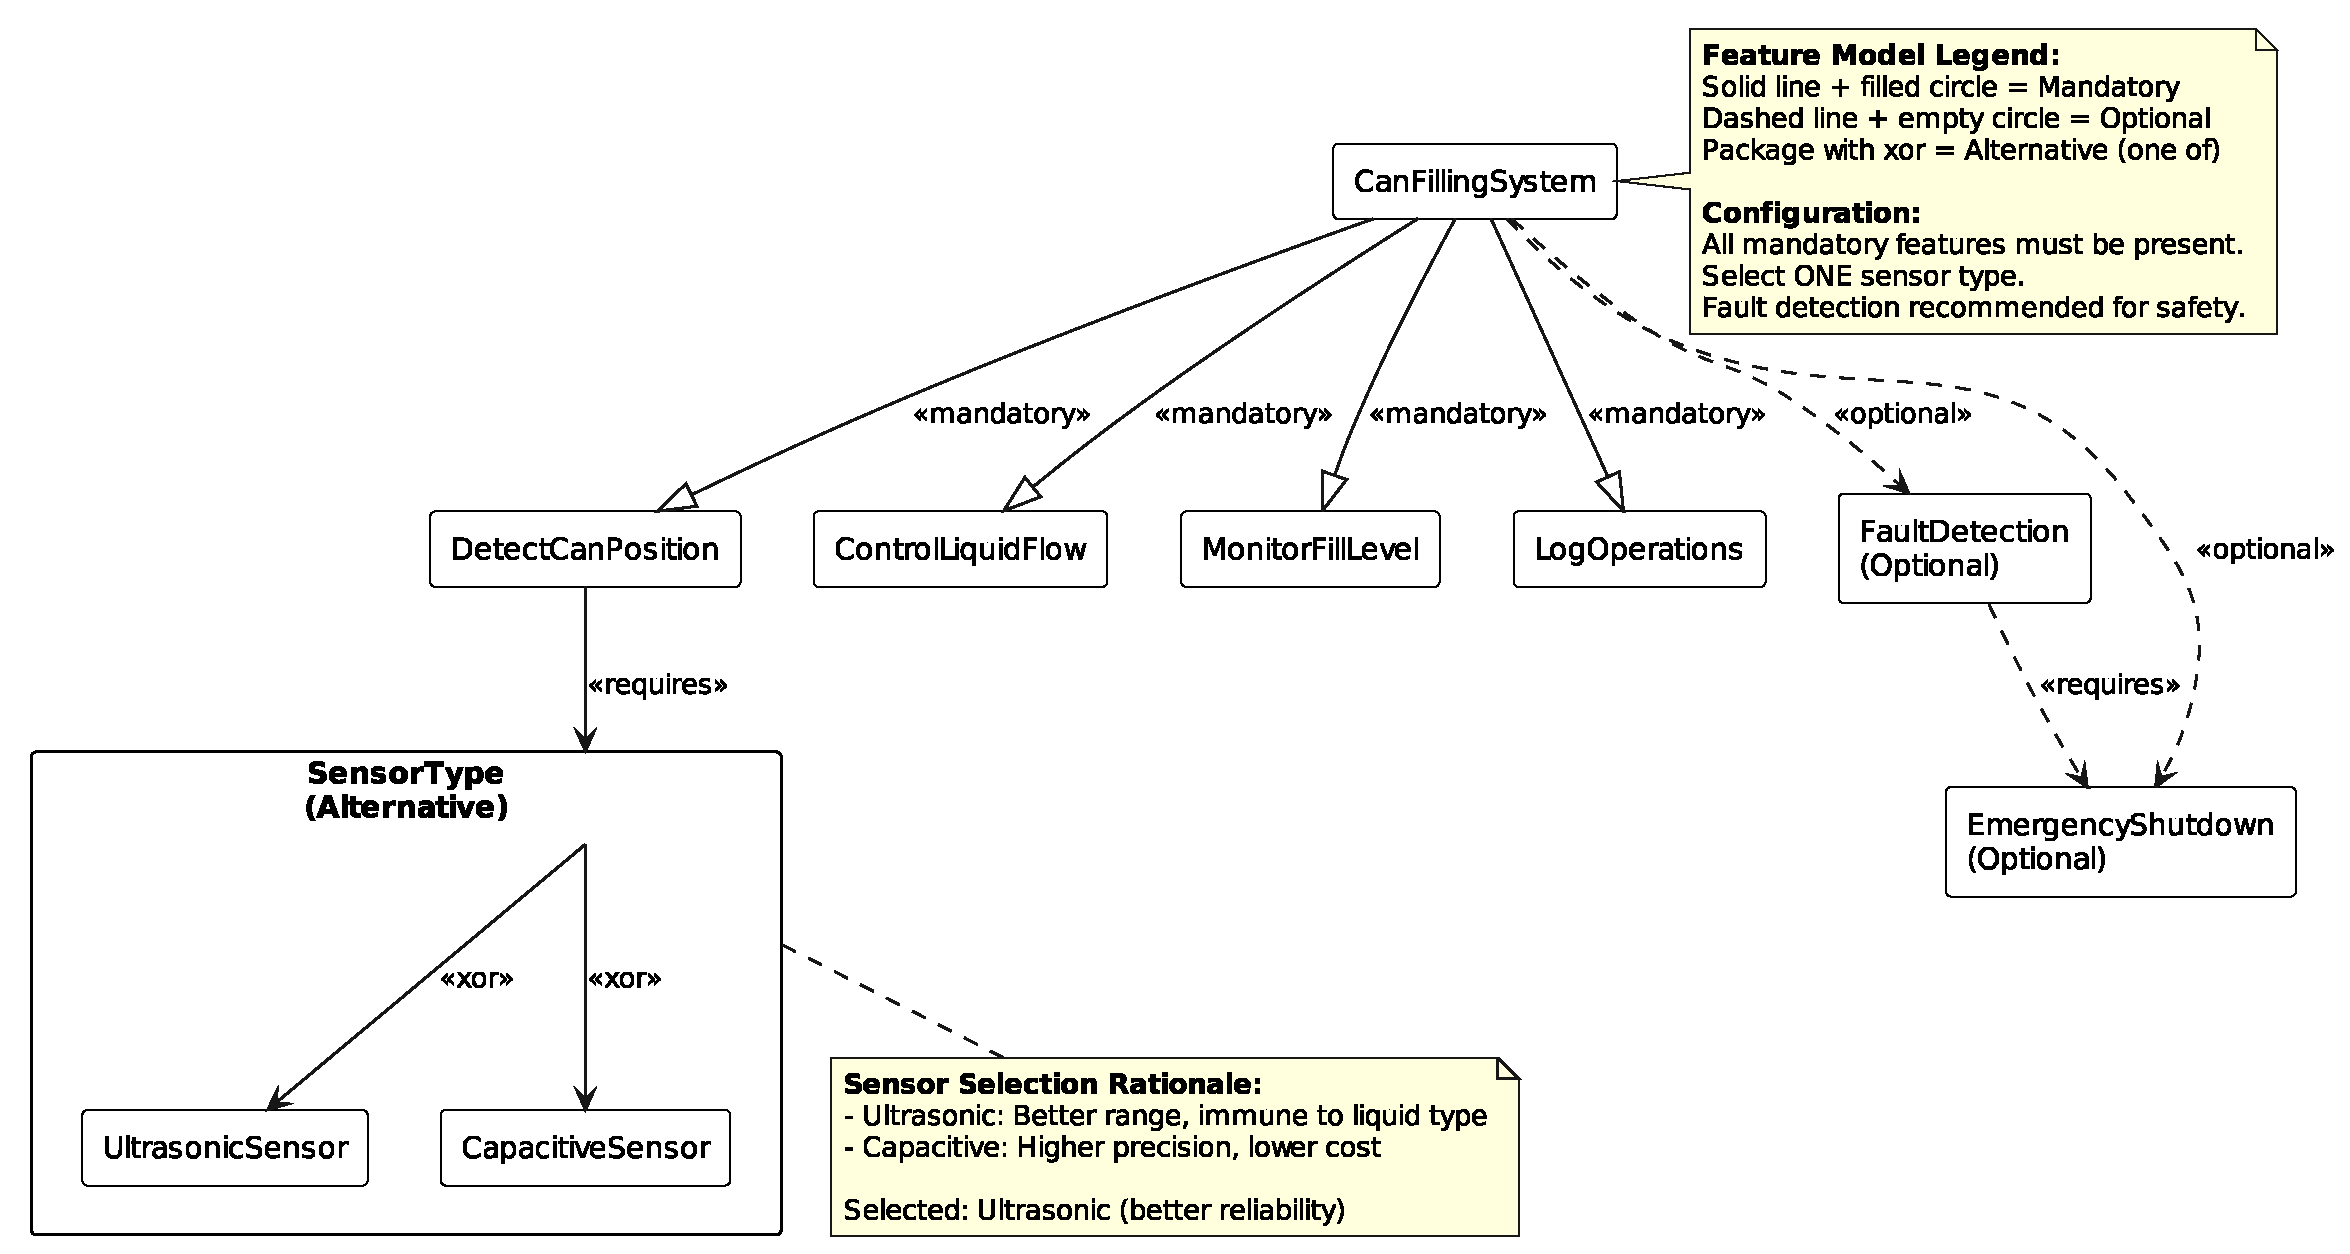
\includegraphics[width=0.48\textwidth]{figures/feature_model.eps}
\caption{Feature model showing mandatory, optional, and alternative features}
\label{fig:features}
\end{figure}

\subsection{Analysis Architecture}

Figure~\ref{fig:components} shows the analysis-level architecture using SysML internal block diagram notation. Three analysis functions comprise the logical architecture:

\textbf{SensorDataCollector:} Polls position and level sensors at 20Hz (50ms intervals), validates readings against tolerance thresholds, and publishes data to MQTT topics. Ports include \textit{sensorInput}, \textit{positionData} (out), \textit{levelData} (out), and \textit{faultSignal} (out).

\textbf{FillController:} Implements the main state machine managing fill cycles. Subscribes to sensor data, commands valve operations, and publishes status updates. Ports include \textit{canPosition} (in), \textit{currentLevel} (in), \textit{valveCommand} (out), and \textit{statusUpdate} (out).

\textbf{FaultHandler:} Monitors fault events across system, classifies severity, and triggers emergency responses. Ports include \textit{faultEvent} (in), \textit{systemState} (in), and \textit{emergencyStop} (out).

\begin{figure}[htbp]
\centering
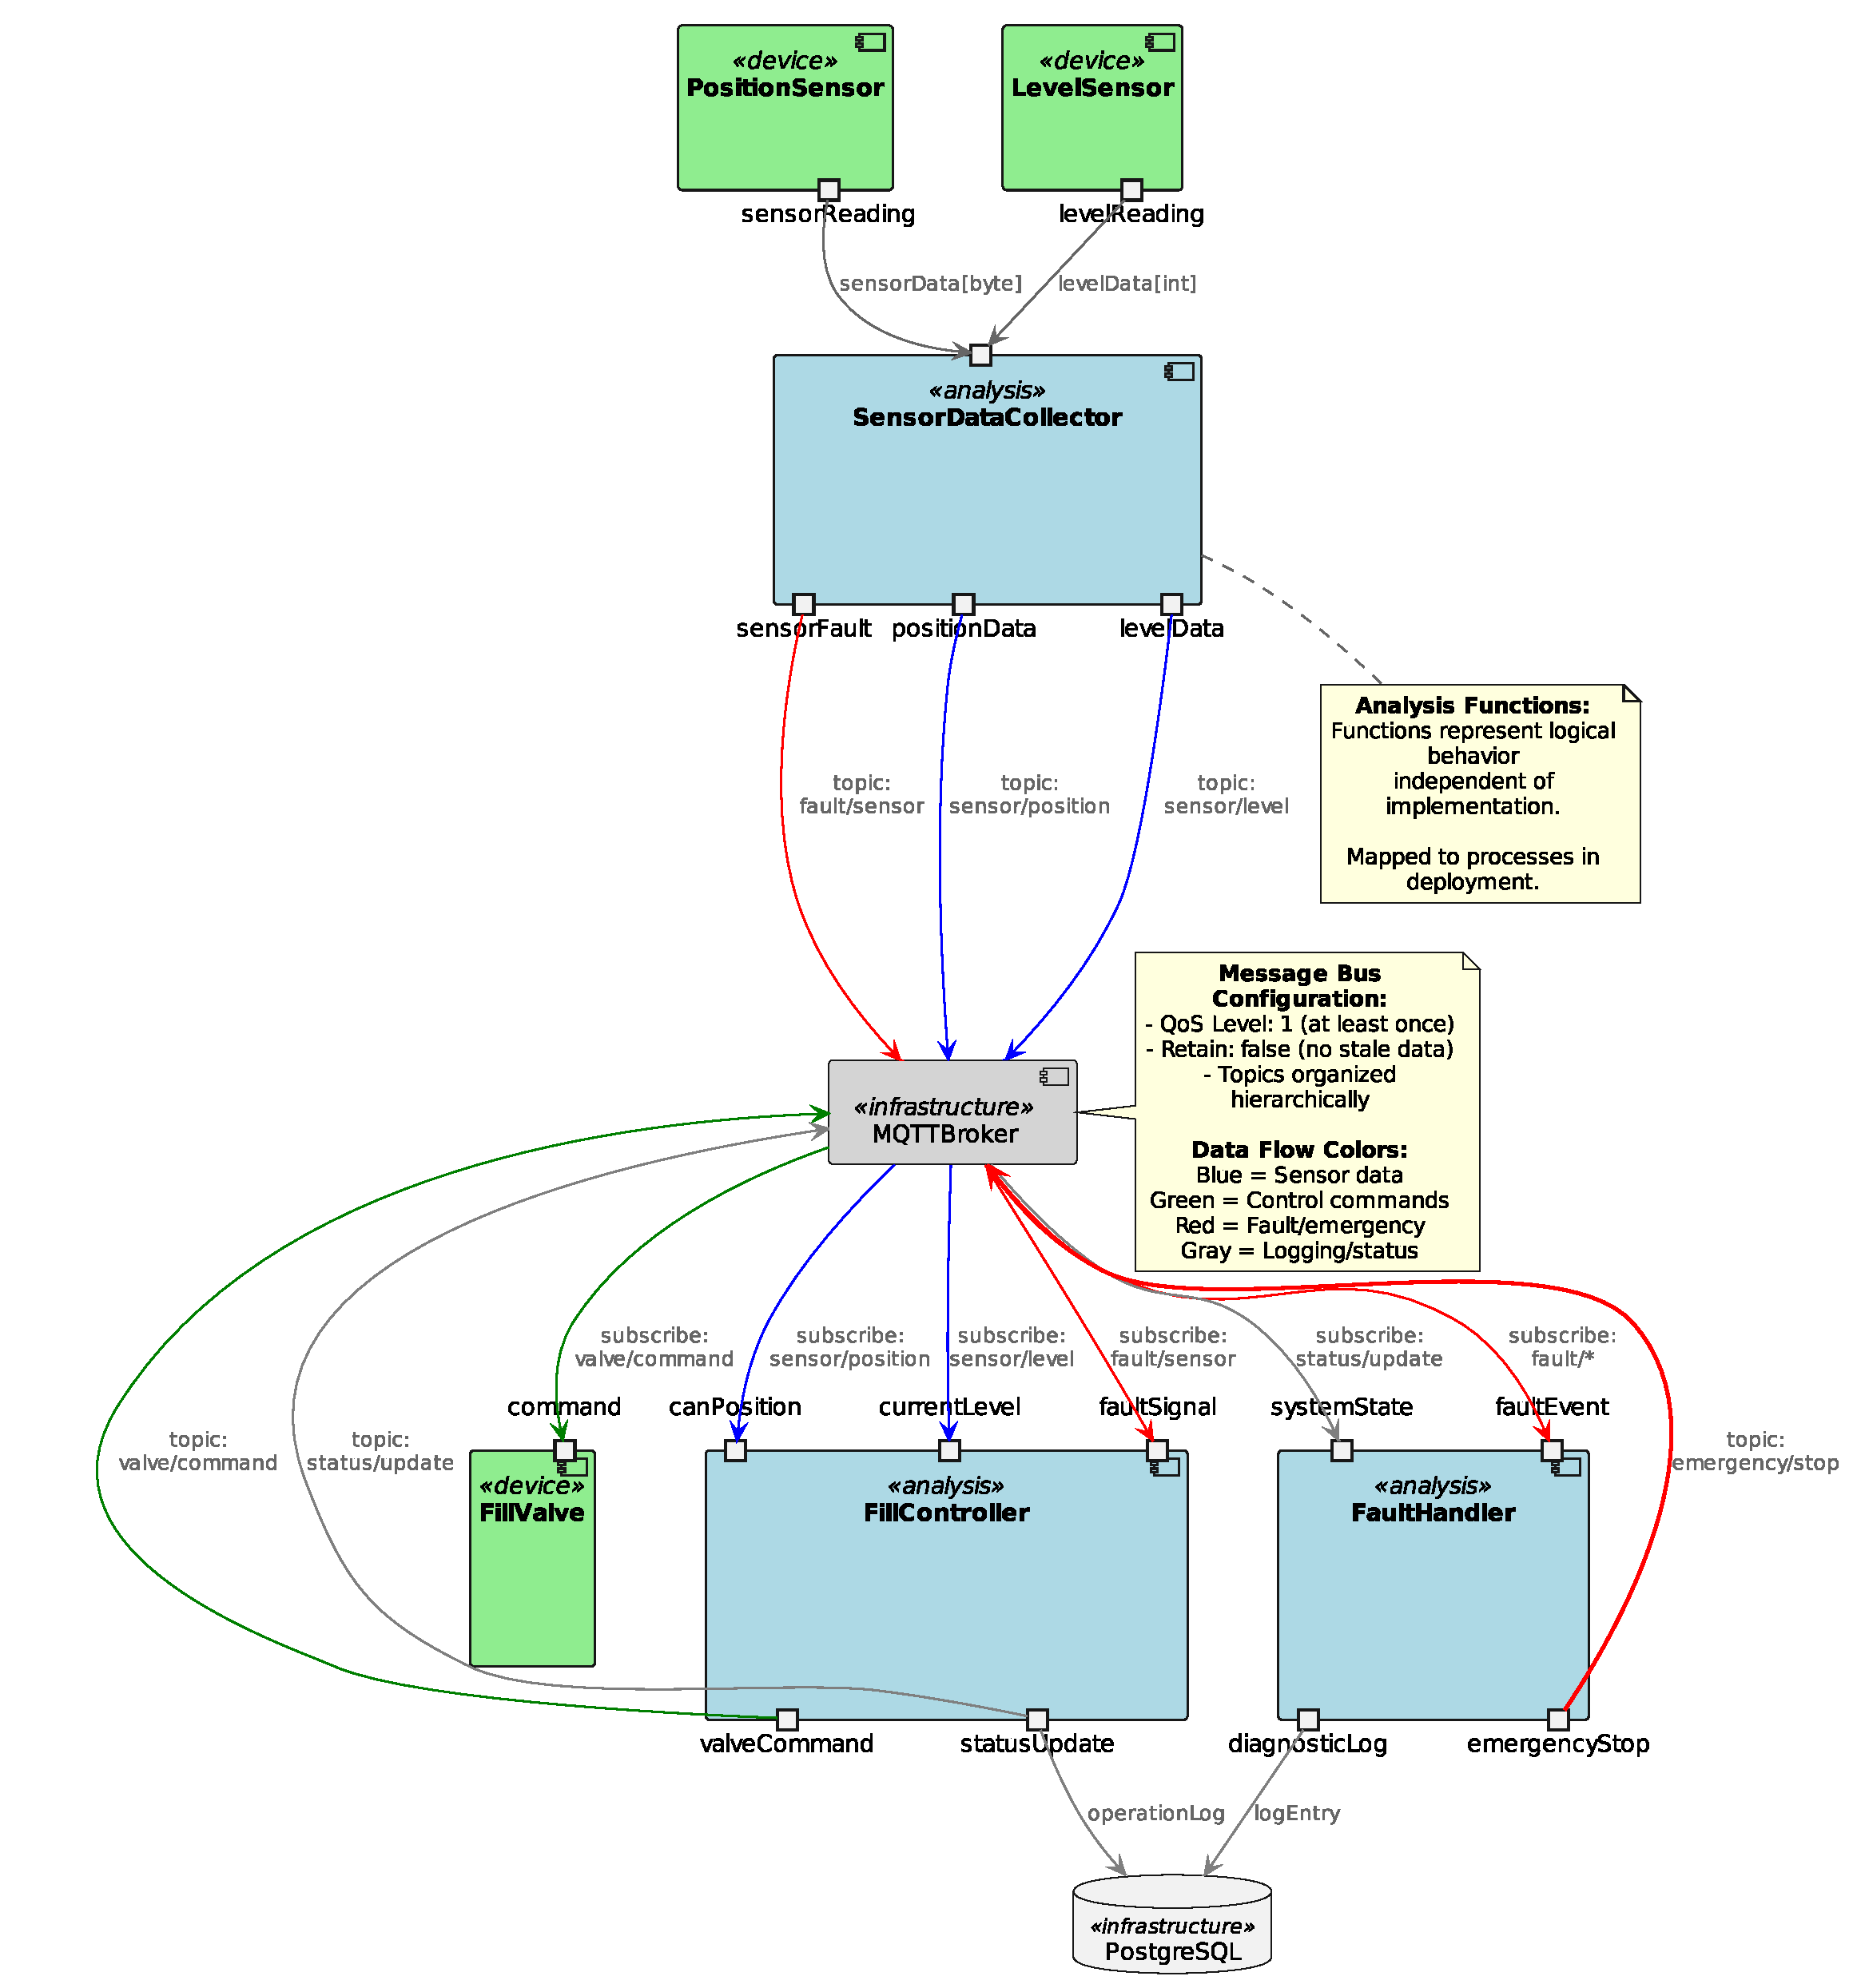
\includegraphics[width=0.48\textwidth]{figures/component_diagram.eps}
\caption{Analysis architecture showing function blocks and data flows via MQTT}
\label{fig:components}
\end{figure}

All communication flows through an MQTT broker configured for QoS 1 (at-least-once delivery), providing loose coupling while ensuring message reliability. Topics follow hierarchical naming: \texttt{sensor/*}, \texttt{valve/*}, \texttt{fault/*}, \texttt{status/*}.

\subsection{Behavioral Models}

Figure~\ref{fig:statemachine} shows the FillController state machine with six states: \textit{Idle}, \textit{WaitingPosition}, \textit{Filling}, \textit{ClosingValve}, \textit{Complete}, and \textit{Fault}.

\begin{figure}[htbp]
\centering
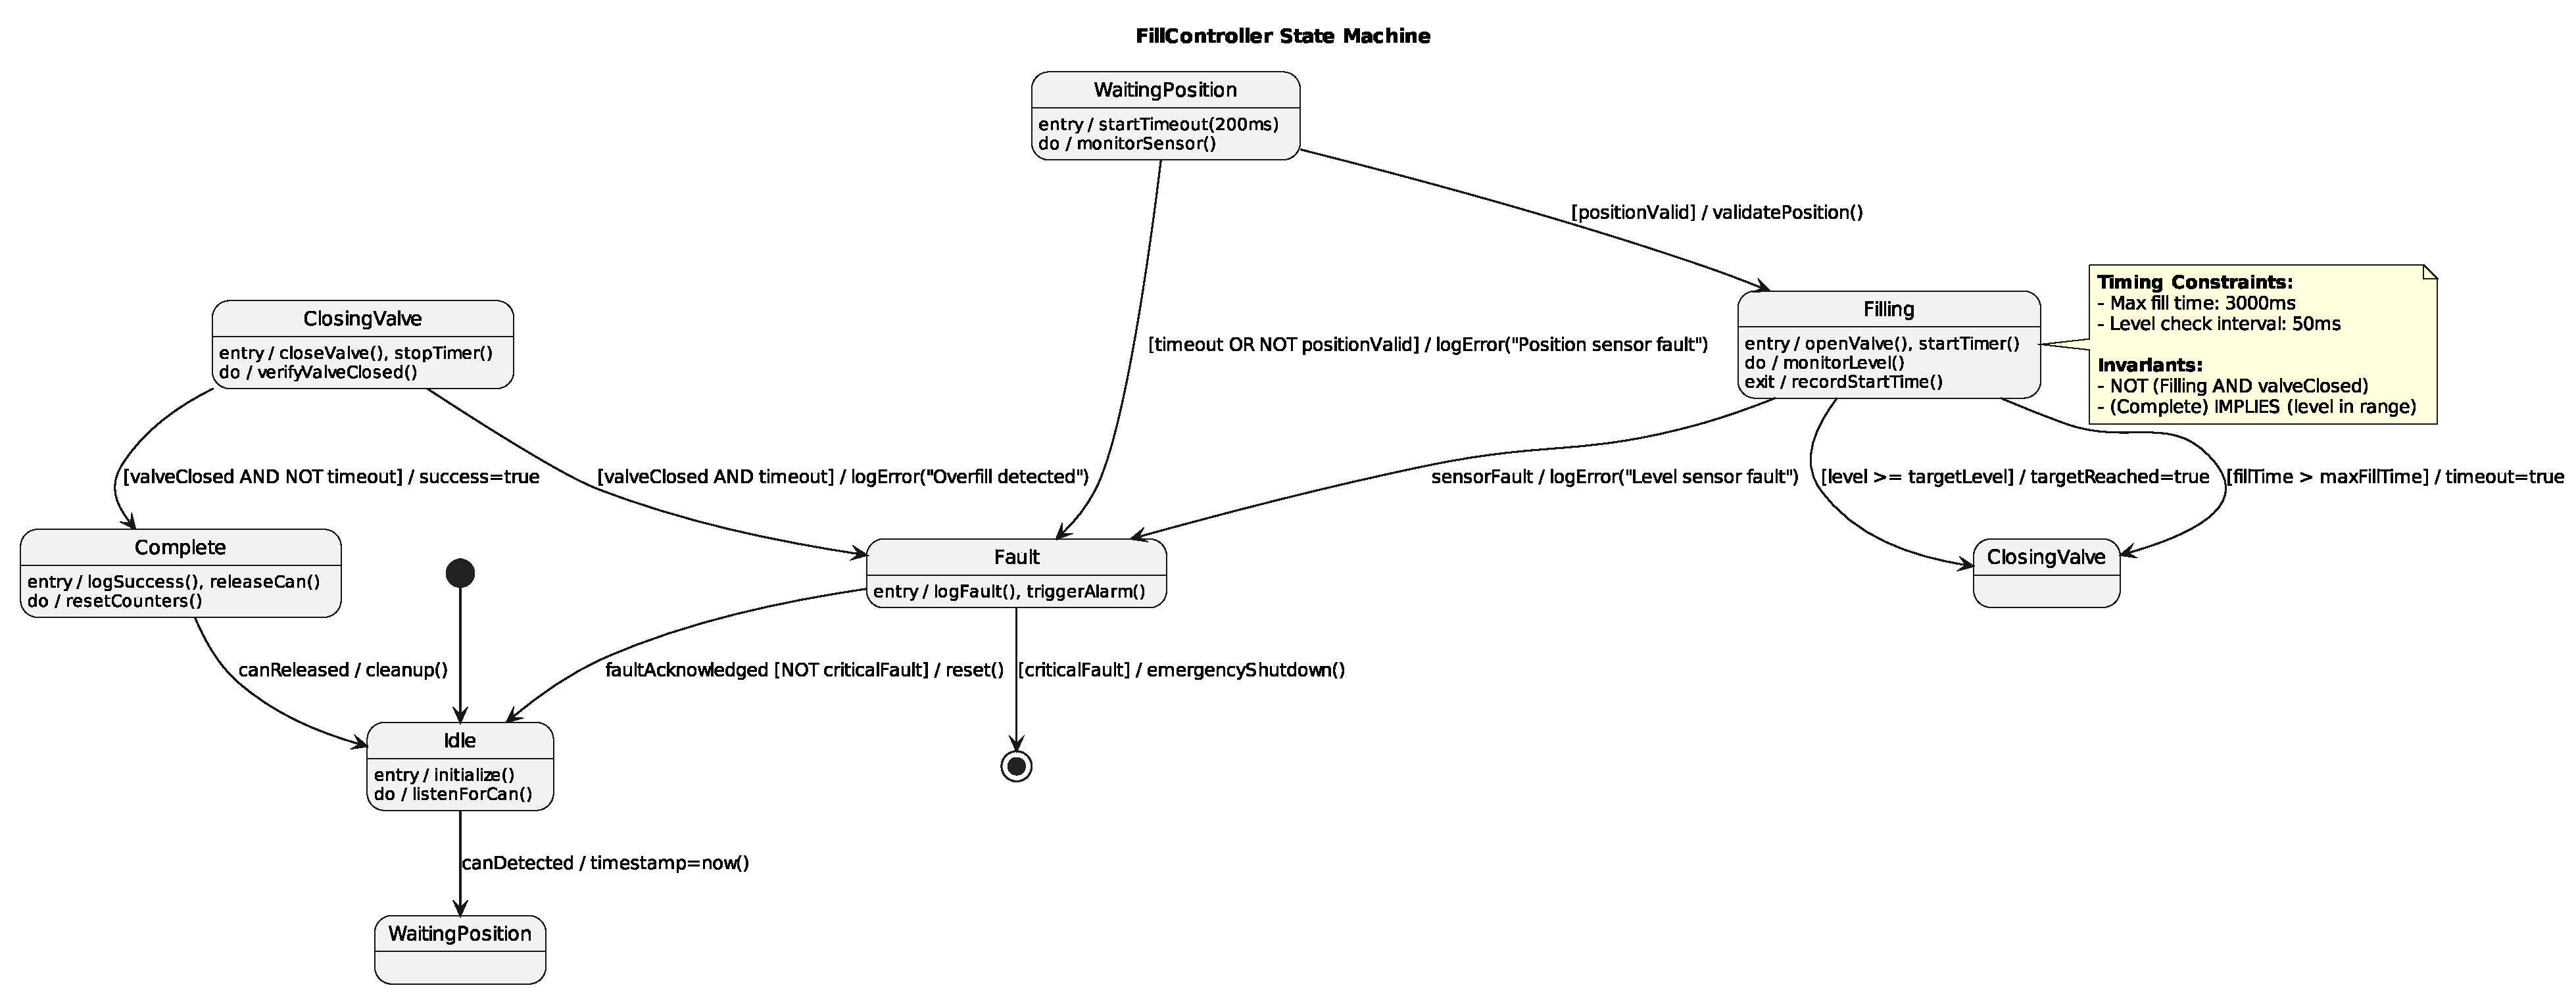
\includegraphics[width=0.48\textwidth]{figures/state_machines.eps}
\caption{FillController state machine with timing guards and invariants}
\label{fig:statemachine}
\end{figure}

Transitions include guards and actions following SysML notation:
\begin{itemize}
    \item \textit{Idle} -> \textit{WaitingPosition} [canDetected] / cycleStart()
    \item \textit{WaitingPosition} -> \textit{Filling} [positionValid AND cycleTime $\leq$ 200ms] / openValve()
    \item \textit{Filling} -> \textit{ClosingValve} [level ≥ 325ml AND fillTime $\leq$ 3000ms] / closeValve()
    \item \textit{ClosingValve} -> \textit{Complete} [levelInTolerance] / logSuccess()
    \item Any state -> \textit{Fault} [timeout OR sensorFailure] / emergencyClose()
\end{itemize}

Timing constraints appear as state invariants (\textit{WaitingPosition}: cycleTime $\leq$ 200ms, \textit{Filling}: fillTime $\leq$ 3000ms) and transition guards, enabling direct mapping to UPPAAL clock constraints.

\subsection{Architectural Decisions and Trade-offs}

\textbf{Decision 1: Event-Driven vs Time-Triggered Architecture}

\textit{Choice:} Event-driven with MQTT asynchronous messaging.

\textit{Rationale:} Enables loose coupling between components, allowing independent development and testing. Components react to events rather than polling on fixed schedules, improving resource utilization.

\textit{Trade-off:} Sacrificed deterministic timing of time-triggered approach for flexibility. Event ordering depends on message broker behavior rather than fixed schedule.

\textit{Mitigation:} Timeout guards in state machine ensure maximum latencies. UPPAAL verification confirms timing bounds are met despite asynchronous communication.

\textbf{Decision 2: MQTT QoS Level}

\textit{Choice:} QoS 1 (at-least-once delivery).

\textit{Rationale:} Balances reliability and latency. QoS 0 (at-most-once) risks message loss during network hiccups. QoS 2 (exactly-once) introduces additional round-trips increasing latency.

\textit{Trade-off:} Possible duplicate messages vs guaranteed delivery. Adds 5-10ms latency compared to QoS 0.

\textit{Mitigation:} Message handlers designed to be idempotent. Empirical testing (Section~\ref{sec:evaluation}) confirms latency remains within bounds.

\textbf{Decision 3: Containerized deployment_architecture}

\textit{Choice:} Docker containers for each component.

\textit{Rationale:} Isolation enables independent scaling, simplified deployment_architecture, and consistent environments across development and production.

\textit{Trade-off:} Container overhead (~10ms startup, small memory cost) vs deployment_architecture flexibility and reproducibility.

\textit{Validation:} Empirical measurements show overhead acceptable for 600-1500ms cycle time requirement.

\subsection{Tactics Applied}

Following Bass et al.~\cite{bass_swa}, we applied specific architectural tactics:

\textbf{Performance:} Asynchronous messaging avoids blocking. 20Hz sensor polling balances responsiveness and CPU usage.

\textbf{Safety:} Timeout watchdogs detect stuck states. Emergency shutdown path bypasses normal control flow.

\textbf{Reliability:} Redundant fault detection at multiple levels. Comprehensive event logging enables post-hoc analysis.

\textbf{Maintainability:} Loose coupling via message bus. Clear interfaces defined by topic schemas.

\textbf{Testability:} Event logs in PostgreSQL provide trace data. Sensor simulator enables controlled testing without physical hardware.
